\chapter{Clases}
\section{Diagrama de clases}
\begin{landscape}
\begin{figure}
\centering
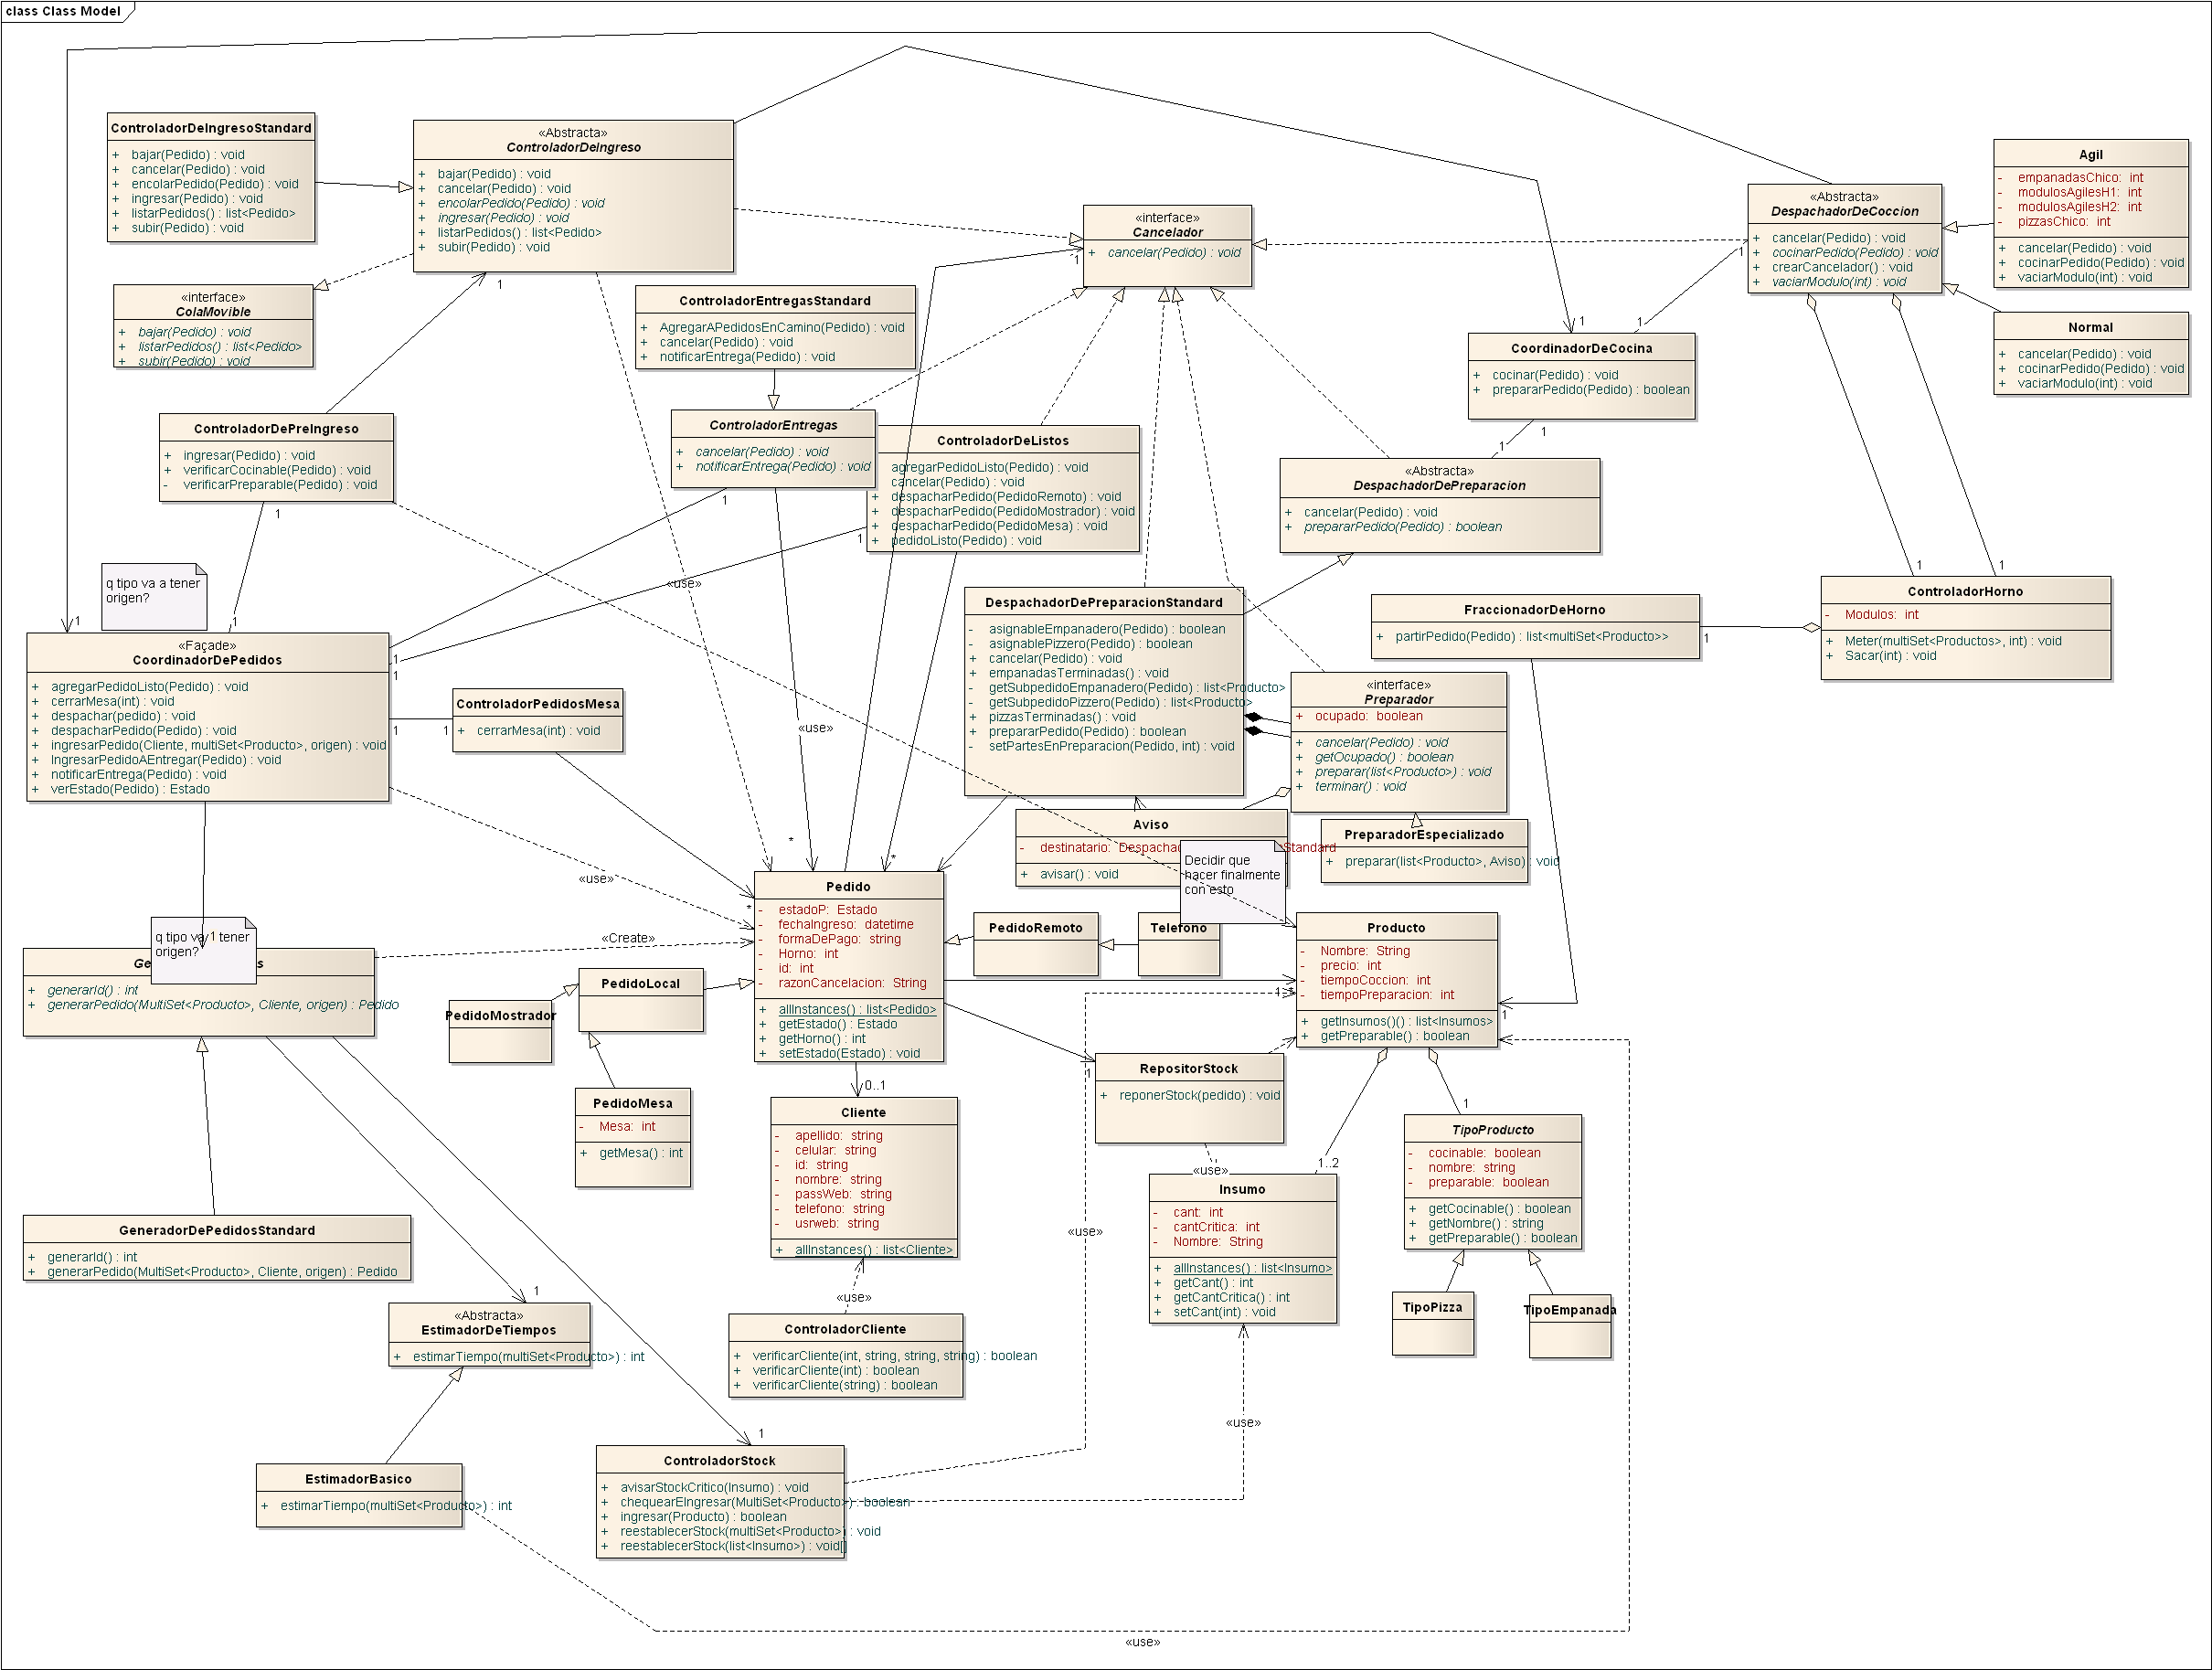
\includegraphics[height=18cm]{./figuras/clases.png}
\end{figure}
\end{landscape}

\section{Explicaci�n de las clases}
\clase
{ABMproductos}
{Esta clase se encarga de realizar las altas, bajas y modificaciones de los productos}
{}{}

\clase
{ABMstock}
{Esta clase se encarga de realizar las altas, bajas y modificaciones de los insumos}
{}{}

\clase
{Agil}
{Especializaci�n de gestor de horno, permite aplicar la politica agil}
{}{}

\clase
{Aviso}
{Clase utilizada para realizar el \textit{callback} desde el gestor de horno hacia el despachador de preparaci�n, es la encargada de ejecutar el metodo del despachador que lo notifica de que se termino de preparar algo. Esta clase permite que el despachador no necesite saber quien le avisa, y por lo tanto permite que los preparadores no requieran de metodos diferenciados para avisar que se terminaron de preparar las pizzas, o las empanadas}
{}{}

\clase{Cliente}
{Esta clase representa a un cliente, conteniendo todos los datos del mismo.}
{}{}

\clase{ColaListos} %FIXME: nombre poco feliz
{Esta clase contiene a los pedidos que ya estan listos. Su responsabilidad es la de conocer a todos los que estan en este estado, a fin de que despachar un pedido se haga desde esta clase}
{}{}

\clase
{ControladorDeIngreso}
{Controla la cola de ingreso, la cual puede ser modificada por el encargado de pedidos. Cuando algun preparador queda libre, envia el proximo pedido a preparar}
{}{}

\clase
{ControladorCliente}
{El controlador de cliente tiene por responsabilidad encargarse de autentificar un usuario}
{}{}

\clase
{ControladorStock}
{El controlador de stock, tiene por responsabilidad chequear la disponibilidad de insumos al momento de un ingreso, asi como la de hacer el decremento del stock al ingresar un pedido, generando el aviso de stock critico en caso de ser necesario.}
{}{}

\clase
{CoordinadorDePedidos}
{El coordinador de pedidos se encarga de controlar el ingreso de pedidos, y su ciclo de vida fuera de la cocina}
{}{}

\clase
{DespachadorDePreparaci�n}
{Esta clase tiene por responsabilidad manejar la cola de pedidos que se estan preparando, recordemos que puede existir una cola de preparaci'on si hay pedidos mixtos a la espera de uno de los maestros. El controlador de ingresos distribuye los pedidos a los distintos preparadores y despacha cada pedido a su gestor de horno correspondiente cuando ya esta preparado.}
{}{}

\clase
{EstimadorDeTiempos}
{El estimador de tiempos, como lo dice su nombre, se encarga de estimar el tiempo de preparacion y cocci�n de un pedido}
{}{}

\clase
{GeneradorDePedidos}
{Esta clase se encarga de crear pedidos, creando pedidos de solo bebidas o con comida segun los productos}%FIXME: justificacion
{}{}

\clase
{GestorHorno}
{Clase abstracta que permite implementar diferentes politicas para el manejo del horno}
{}{}

\clase
{Insumo}
{Contiene la informaci�n de los distintos insumos de la pizzer�a}
{}{}

\clase
{Normal}
{Permite implementar la politica normal de manejo del horno}
{}{}

\clase
{Pedido}
{Contiene la informaci�n de cada pedido}
{}{}

